\documentclass[hidelinks]{ctexart}

\usepackage[sensei=陈向军/刘明辉,gakka=原子物理学,gakkabbr=AP]{styles/kurisu}
\usepackage{van-de-la-illinoise}

\begin{document}

\showtitle{原子物理学}

\seclink{sec:sec1}{原子模型と水素様原子}
\seclink{sec:sec2}{量子力学}
\seclink{sec:sec3}{電子のスピンと微細構造}
\seclink{sec:sec4}{多電子原子}
\clearpage
\phantomsection\label{sec:sec1}
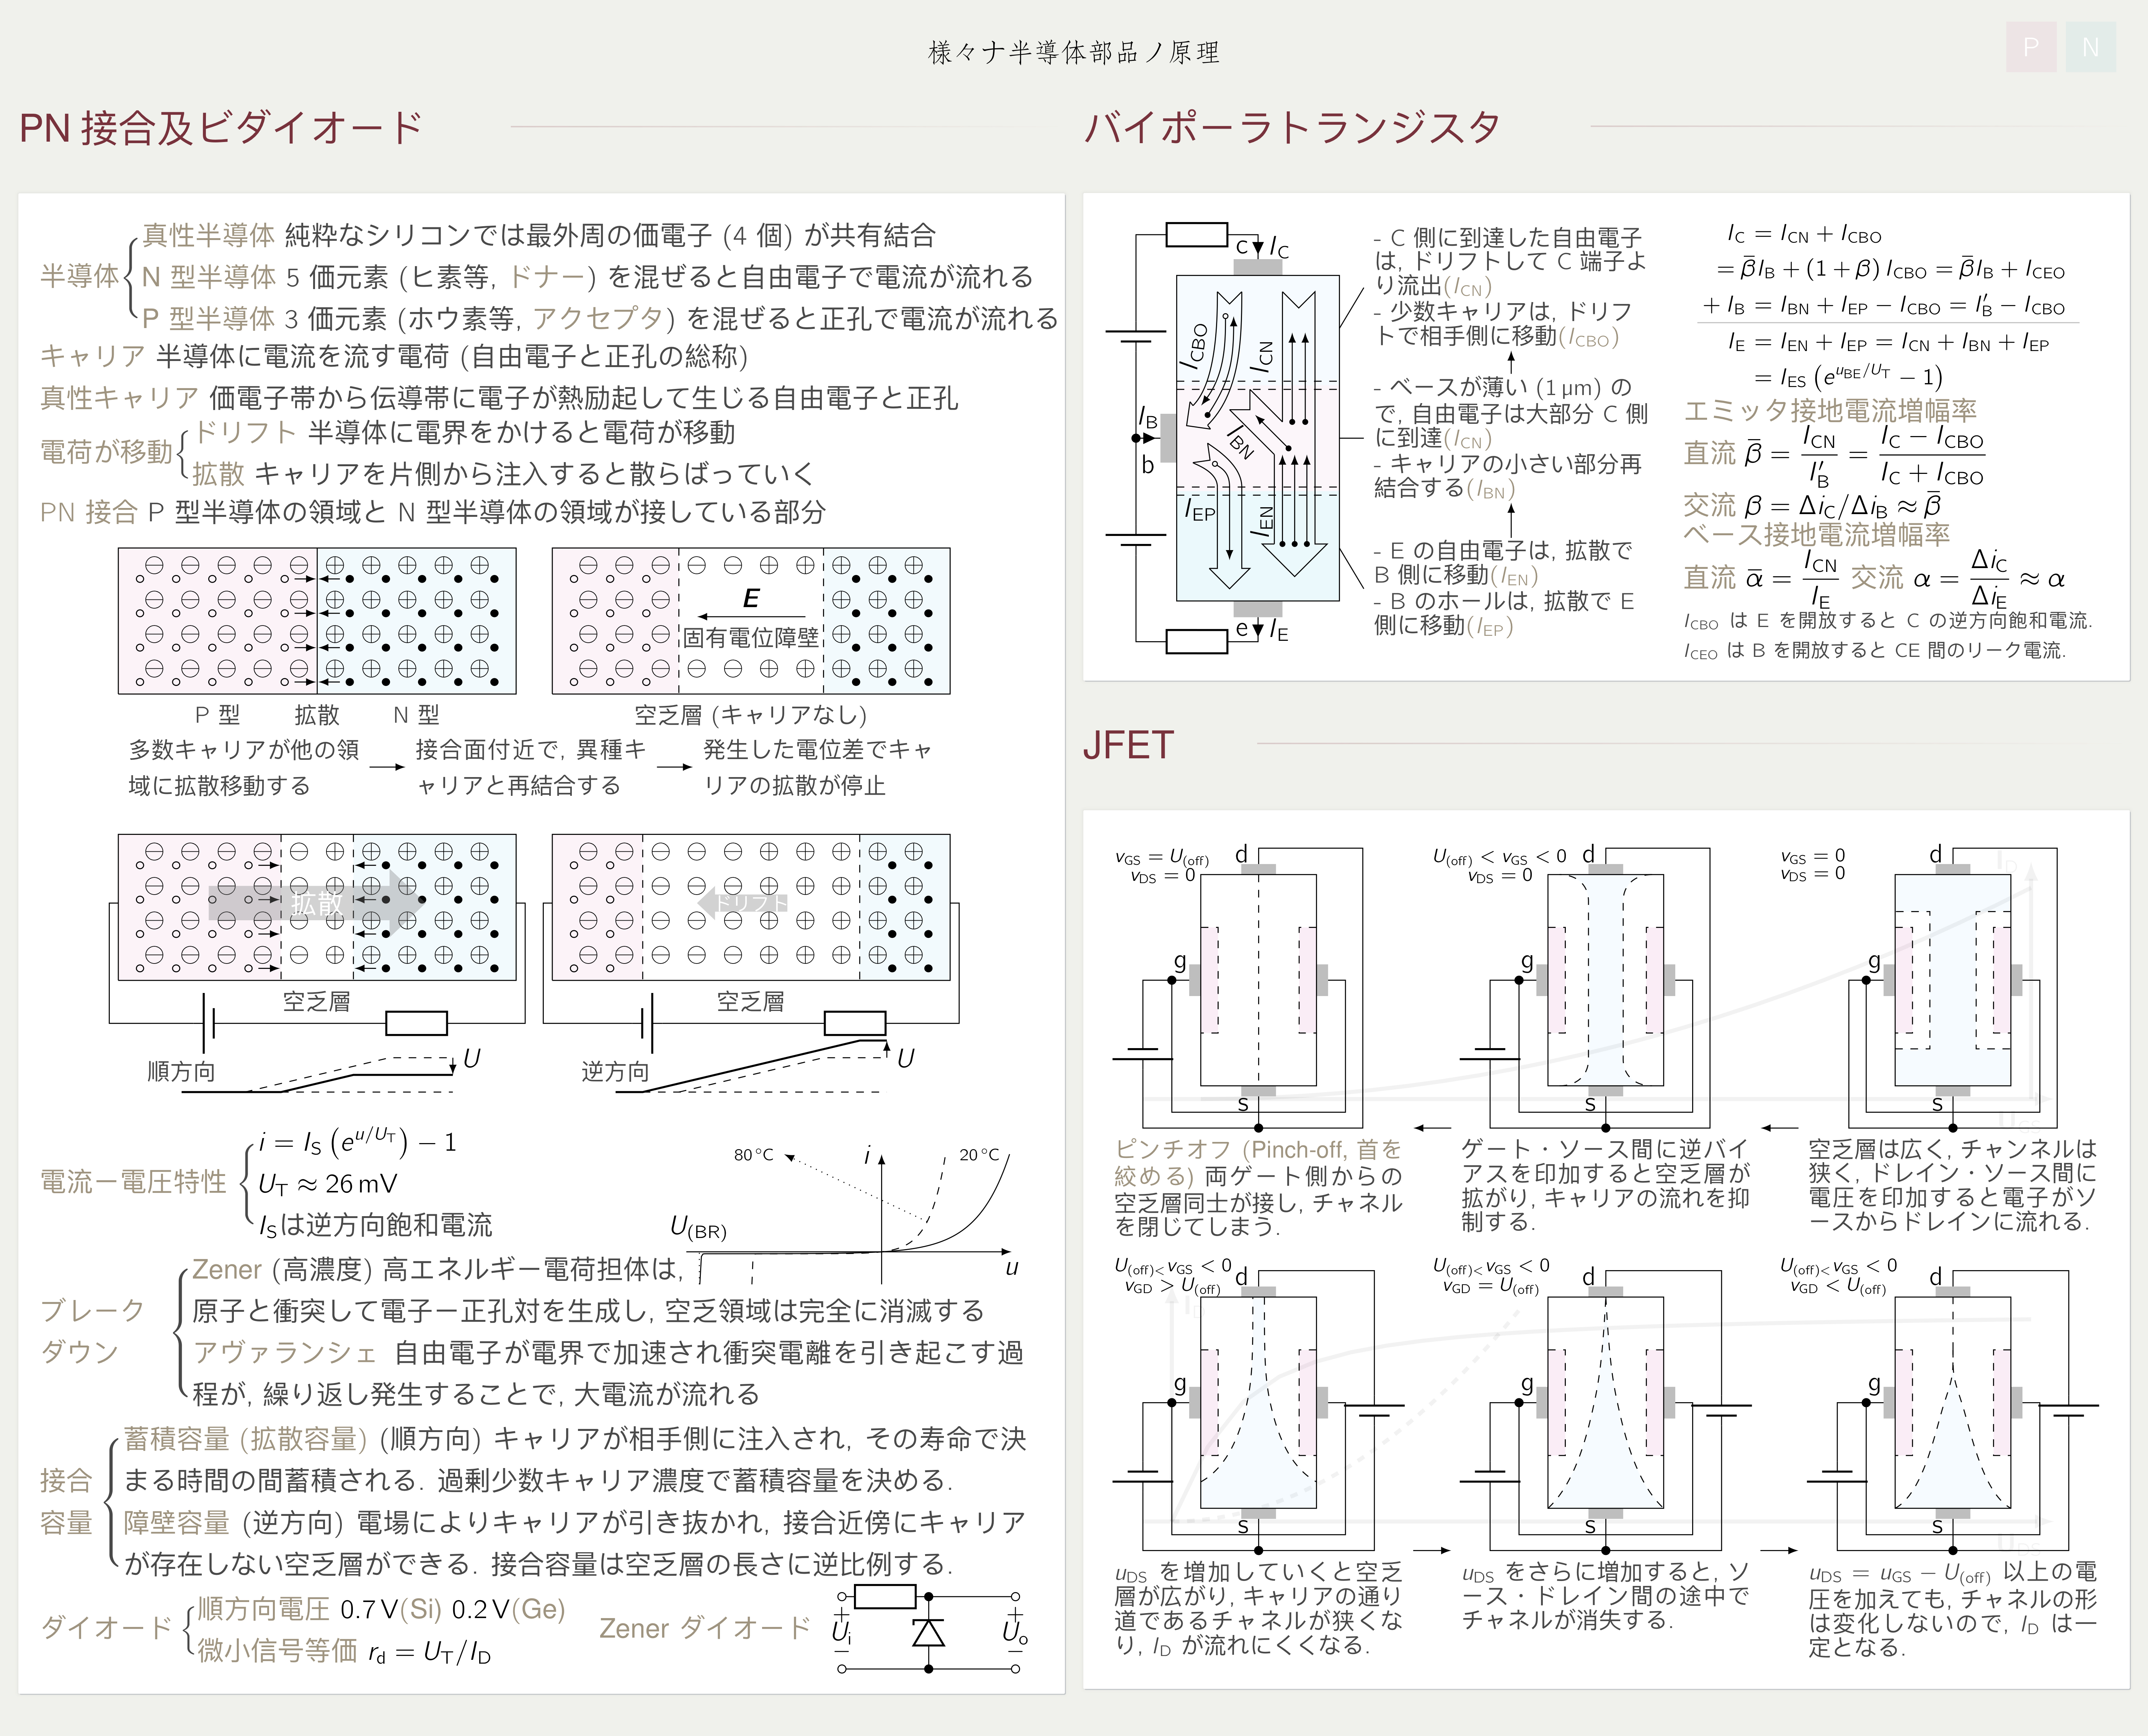
\includepdf[link,pages=-]{Elementary/Elementary.pdf}
\clearpage
\phantomsection\label{sec:sec2}
\includepdf[pages=-]{Quantum/Quantum.pdf}
\clearpage
\phantomsection\label{sec:sec3}
\includepdf[pages=-]{FineStructure/FineStructure.pdf}
\clearpage
\phantomsection\label{sec:sec4}
\includepdf[pages=-]{Multielectron/Multielectron.pdf}

\end{document}
